\documentclass[a4paper, 12pt]{article}
\usepackage[a4paper, left=0.4cm, right=0.4cm, top=0.3cm, bottom=0.5cm, landscape]{geometry}
\usepackage{multicol}
\usepackage{listings}
\usepackage{enumitem}
\usepackage{graphicx}
\usepackage{courier}
\usepackage{vwcol}
\usepackage{amsmath}
\usepackage[super]{nth}

\setitemize{noitemsep,topsep=0pt,parsep=0pt,partopsep=0pt,leftmargin=*}
\setenumerate{noitemsep,topsep=0pt,parsep=0pt,partopsep=0pt,leftmargin=*}
\lstset{
	belowskip=0.1em,
	aboveskip=0.1em,
    basicstyle=\ttfamily,
}

\begin{document}
\setlength\parindent{0pt}
\setlength{\multicolsep}{1.0pt plus 2.0pt minus 1.5pt}% 50% of original values
\scriptsize
\pagenumbering{gobble}

\begin{center}
{\normalsize\textbf{CS2106 Cheatsheet 19/20 S1 Finals}}
\end{center}
\begin{multicols*}{4}
\noindent
{\small\textbf{Introduction}}
\begin{itemize}
	\item Data: global variables
	\item Text: raw source code/instructions
	\item Stack: args/params/local vars/caller return addr
	\item Heap: dynamically allocated with \texttt{malloc}
\end{itemize}
\textbf{Stack Frame Setup/Teardown} \\
On executing function call:
\begin{itemize}
    \item Caller: Pass arguments with Registers/Stack
    \item Caller: Save return PC on Stack
    \item Transfer control from caller to callee
    \item Callee: Save registers used by callee and old FP/SP
    \item Callee: Alloc space for local vars of callee on stack
    \item Callee: Adjust SP to point to new stack top
\end{itemize}
On returning from function call:
\begin{itemize}
    \item Callee: Restore saved Registers, FP, SP
    \item Transfer control from callee to caller
    \item Caller: Continues execution in caller
\end{itemize}

\medskip

{\small\textbf{Process Abstraction}}
\begin{itemize}
	\item Exceptions: synchronous; due to program
	\item Interrupts: asynchronous; independent of program
	\item Memory Context: text, data, stack, heap
	\item Hardware Context: registers, PC, SP, FP
	\item OS Context: PID, process state, opened files
	\item PCB: stores all contexts of an executing process
	\item \texttt{exec()}: replaces current process with new process
\end{itemize}
\textbf{Fork}
\begin{itemize}
	\item child $\rightarrow$ \texttt{fork() == 0}; parent $\rightarrow$ \texttt{fork() > 0}
	\item Data is copied, not shared
\end{itemize}
\begin{itemize}
	\item \texttt{exit(status)} causes value of \texttt{status} to be returned to the parent's call to \texttt{wait(\&status)}. 8 LSB is exit status (\texttt{pid = status>>8})
\end{itemize}
\textbf{Zombie Process}
\begin{itemize}
	\item Child process that has completed execution (\texttt{exit} system call) but still has an entry in the process table (so parent process can still read exit status)
	\item \texttt{kill} command has no effect on a zombie process
\end{itemize}
\textbf{Orphan Process}
\begin{itemize}
	\item Parent terminated, but child still executing
	\item Dead orphan processes waited on by init (PID 1)
\end{itemize}

\medskip

\begin{minipage}{.33\linewidth}
	{\small\textbf{Process \\ Scheduling}}
\end{minipage}
\begin{minipage}{.66\linewidth}
	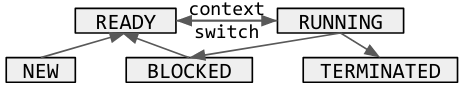
\includegraphics[scale=0.3]{5-state.png}
\end{minipage}
\begin{itemize}
	\item Non-preemptive/Cooperative: B will wait for A to finish (or be blocked) before B starts running
	\item Preemptive: suspend process after time quantum
	\item Burst Time: time spent actually using CPU
	\item Turnaround Time: end time - enqueue time
	\item Response Time: start time - enqueue time
	\item Waiting Time: turnaround time - burst time
	\item Throughput: \# tasks finished per unit time
\end{itemize}
\textbf{Batch Processing}
\begin{itemize}
	\item No user interaction, no need to be responsive
	\item Prioritises turnaround/burst time, throughput
\end{itemize}
\textbf{First Come First Served (FCFS)}
\begin{itemize}
	\item FIFO queue; any process will eventually run
	\item Blocked process is added back to queue when ready
	\item Convoy Effect: short tasks waiting for a long task
\end{itemize}
\textbf{Shortest Job First (SJF)}
\begin{itemize}
	\item Select task with smallest \textbf{total} CPU time
	\item OS needs to know CPU time for a task in advance
\end{itemize}
\textbf{Shortest Remaining Time First (SRT)}
\begin{itemize}
	\item Select task with smallest \textbf{remaining} CPU time
	\item Will preemptively stop another process to allow the shorter remaining time task to run
\end{itemize}
\textbf{Interactive Processing}
\begin{itemize}
	\item Prioritises response time, and predictability
\end{itemize}
\textbf{Round Robin (RR)}
\begin{itemize}
	\item Preemptive version of FCFS
	\item Each process given a pre-defined time quantum
	\item After using up time quantum, if task is not yet finished, task gets put back in back of queue
\end{itemize}
\textbf{Priority Scheduling}
\begin{itemize}
	\item Do tasks with highest priority first
	\item Hard to guarantee exact amount of CPU time given to each process; low priority tasks may be starved
	\item May lead to priority inversion: \\
		$P(H) > P(M) > P(L)$. $L,H$ shares CS but neither with $M$. $L$ is running in CS. $H$ also needs to run in CS. $H$ waits for $L$ to come out of CS. $M$ able to interrupt $L$ and starts running. $M$ runs till completion. $L$ resumes and starts running till the end of CS. $H$ finally enters CS and starts running.
\end{itemize}
\textbf{Multi-Level Feedback Queue (MLFQ)}
\begin{itemize}
	\item If $P(A) > P(B)$, then $A$ runs
	\item If $P(A) = P(B)$, then $A$ and $B$ runs in RR
\end{itemize}
Settings:
\begin{itemize}
	\item New tasks will have highest priority
	\item Time slice is used before finishing task $\Rightarrow P \downarrow$
	\item Task blocks before time slice is used $\Rightarrow P$ same
\end{itemize}

\medskip

{\small\textbf{Inter Process Communication (IPC)}} \\
\textbf{Shared Memory}
\begin{lstlisting}[language=C]
shmat(int shmid, void *shmaddr, int flg);
\end{lstlisting}
\begin{itemize}
	\item Attaches the shared memory segment (\texttt{shmid}) to the address space (\texttt{shmaddr}) of the calling process. If \texttt{shmaddr} is \texttt{null}, attach to first available addr
	\item Region is referred to by \texttt{shmid}, not by \texttt{shmaddr}
	\item Efficient: only the initial attach step involves OS
	\item Ease of use: shared memory behaves as per normal
	\item Hard to synchronise (see Race Condition)
\end{itemize}
\textbf{Message Passing}
\begin{itemize}
	\item Passed message is stored in kernel memory space
	\item Easy to synchronise for synchronous primitives
	\item Inefficient: every send/recv operation involves OS
\end{itemize}
\textbf{UNIX Pipe}
\begin{itemize}
	\item \texttt{A | B} means pipe output of \texttt{A} to input of \texttt{B}
	\item Data must be accessed in order (FIFO)
	\item Implicit synchronisation (waits when empty/full)
	\item Read end: \texttt{0}, write end: \texttt{1}
\end{itemize}
\textbf{Signal}
\begin{lstlisting}[language=C]
signal(int signum, sighandler_t handler);
\end{lstlisting}
\begin{itemize}
	\item \texttt{signal()} sets the disposition of the signal \texttt{signum} to \texttt{handler}: either \texttt{SIG\_IGN} (ignore), \texttt{SIG\_DFL} (default handler), or the address of a defined function
	\item Asynchronous $\rightarrow$ vulnerable to race conditions
	\item Use \texttt{sigwait} to synchronously block till signal recv
\end{itemize}

\medskip

{\small\textbf{Threads}}
\begin{itemize}
    \item \texttt{pthread\char`_create()}: \texttt{0} on success, \texttt{!0} on errors
	\item \texttt{pthread\char`_exit(void *retval)}: terminates the calling thread and returns a value via \texttt{retval}
	\item \texttt{pthread\char`_join(pthread\char`_t t, void **ret)}: waits for \texttt{t} and sets \texttt{ret} to \texttt{t}'s \texttt{retval}
	\item A single thread exits when:
	\begin{itemize}
		\item Calling \texttt{pthread\char`_exit} or \texttt{pthread\char`_cancel}
		\item Returning from \texttt{start\char`_routine}
	\end{itemize}
	\item ALL threads exit when:
	\begin{itemize}
		\item Any thread calls \texttt{exit()} 
		\item Main thread returns from \texttt{main()}
	\end{itemize}
	\item Threads in the same process shares
	\begin{enumerate}
		\item Memory Context: variables, text, data, heap
		\item OS Context: PID, opened files (\texttt{pd}), signals, etc
	\end{enumerate}
	\textbf{*Not shared:} Thread ID, registers, and \textbf{stack}
\end{itemize}
\textbf{Kernel Threads}
\begin{itemize}
	\item Maintains kernel-level thread table
	\item Thread operations are system calls (slower)
	\item Can Thread Switch if threads from \textbf{same} process
\end{itemize}
\textbf{User Threads}
\begin{itemize}
	\item Each process maintains its own private thread table
	\item Thread operations are runtime procedures (faster)
	\item Only Process Switch: threads \textbf{transparent to OS}
\end{itemize}
\textbf{Hybrid Threads}
\begin{itemize}
	\item OS only aware of (and schedules) kernel threads
	\item Multiple user threads can bind to a kernel thread
\end{itemize}
\begin{tabular}{ |c|c| }
    \hline
	\textbf{Process Switch} & \textbf{Thread Switch} \\
	\hline
	Switches full VM space & Switches GPR/PC/stack \\
	Flushes TLB cache & Keeps TLB cache \\
	More overhead & Less overhead \\
	\hline
\end{tabular}
\textbf{Threads vs Processes}
\begin{enumerate}
    \item Memory
    \begin{itemize}
        \item Threads share same memory space
        \item Processes each have independent memory space
        \item Multiprocess is used if memory usage is heavy
        \item Multithreading is cheaper if sharing large data
    \end{itemize}
    \item Overhead: thread creation is cheaper than forking
    \item Protection: processes have independent memory space, child processes can potentially hang, deface memory, without really affecting other processes
    \item Hardware: some do not support multiple threads
    \item OS: some OSes favour one over the other
\end{enumerate}

\medskip

{\small\textbf{Synchronisation}} \\
\textbf{Race Condition}
\begin{lstlisting}
lw   $r1, var    # init var as 0
addi $r1, $r1, 3 
sw   $r1, var
\end{lstlisting}
Only 2 possible outcomes, \texttt{var} is \texttt{3} or \texttt{6}:
\begin{enumerate}
	\item Both threads \texttt{lw} from \texttt{var} simultaneously (ie. both loads \texttt{0} to \texttt{\$r1}) and eventually \texttt{sw 3} to \texttt{var}
	\item One thread finishes and \texttt{sw 3}. The other thread then starts executing, and finishes to \texttt{sw 6} to \texttt{var}
\end{enumerate}
\textbf{Critical Section (CS)} \\
Properties to maintain:
\begin{itemize}
	\item Mutual Exclusion: exactly one process in CS
	\item Progress: if no processs, one should enter
	\item Bounded Wait: process must eventually enter
	\item Independence: process not executing in CS should never block other processes waiting to enter
\end{itemize}
Incorrect use can lead to deadlock/livelock/starvation \\
\textbf{Test \& Set}
\begin{enumerate}
	\item Atomically set \texttt{1} to memory and return old value
	\item If old value is \texttt{1}, repeat step 1 (busy wait)
	\item When exiting CS, set memory/lock to \texttt{0}
\end{enumerate}
\textbf{Semaphore} \\
Counter \& waiting list (may not be FIFO) of processes
\begin{itemize}
	\item \texttt{wait(S)}: decrement $counter$ by 1. If $counter < 0$, add process to waiting list and block self
	\item \texttt{signal(S)}: increment $counter$ by 1. If $counter \leq 0$, resume/remove a process from waiting list
\end{itemize}
\begin{enumerate}
	\item $-counter$ is the number of waiting processes
	\item \texttt{signal()} is never blocked, but \texttt{wait()} may
	\item \texttt{wait()} and \texttt{signal()} must be \textbf{atomic}
	\item Deadlock is still possible with incorrect use
\end{enumerate}

\setlength{\columnsep}{-1.4cm}
\begin{multicols}{2}
\noindent
\begin{lstlisting}[language=C]
semaphore S = 3;
while (1)
    S.wait();
    // CS
    S.signal();
\end{lstlisting}
\vfill\null
\columnbreak
At most 3 processes can be in CS before CS is locked. Only when a process in CS finishes the work and calls \texttt{signal()} can another process enter CS.
\end{multicols}

{\small\textbf{Memory Management}} \\
\textbf{Buddy System Allocation (RAM)}\\
To allocate memory:
\begin{enumerate}
	\item Look for smallest $2^k$ block $\geq$ requested memory, $R$
	\item If found, allocate it
	\item Else, split a free memory slot $> R$ by half
	\begin{enumerate}
		\item[1.] If lower limit is not reached, repeat step 3
		\item[2.] Else, allocate it
	\end{enumerate}
\end{enumerate}
To deallocate memory:
\begin{enumerate}
	\item Free the block
	\item Determine if neighbour blocks are free
	\item If free, combine the two and repeat step 2 till upper limit reached or non-free neighbour encountered
\end{enumerate}
\textbf{Problems With Physical Memory (PM)} \\
If program can address full 32-bit PM address space,
\begin{enumerate}
	\item Program can crash if RAM $< 2^{32}\text{B} = 4\text{GB}$
	\item Can run out of space if running multiple programs
	\item Can access and corrupt other programs' data
\end{enumerate}
\textbf{Virtual Memory (VM)}
\begin{itemize}
	\item Without VM: program address = RAM address
	\item Maps program address to RAM address
	\item \texttt{printf("\%p")} prints VM address (not PM addr)
\end{itemize}
This solves each problem of PM by,
\begin{enumerate}
	\item Allowing writing to/fro disk when RAM is full
	\item Allowing program data to be anywhere in RAM
	\item Making each program have a different mapping
\end{enumerate}
\textbf{Paging Scheme}
\begin{itemize}
	\item Physical Frame: split regions of physical memory
	\item Virtual Page: split regions of logical memory
\end{itemize}
\textbf{Memory Management Unit (MMU)}
\begin{itemize}
	\item Maps virtual addr to physical memory addr 
	\item Transfers betw RAM/disk always in whole pages
\end{itemize}
\textbf{Page Table}
\begin{itemize}
	\item Maps virtual page num to physical frame num
	\item Virtual page number is used as index to find PTE
	\item Every process stores in RAM its own page table
	\item Size of PTE increases as page/frame size decreases
	\item Size of page table dependent on total VM space
\end{itemize}
Assuming $M$-bit machine with page size $p$B:
\begin{itemize}
	\item Page size = $p$B $\implies$ bits for page offset = $\log_2(p)$
	\item Bits to index PTE = $M-\log_2(p)$
	\item Number of PTEs = $2^{M-\log_2(p)}$
	\item Since PTE = $4$B, page table size = $4(2^{M-\log_2(p)})$B
\end{itemize}
\textbf{Page Fault}
\begin{itemize}
	\item Only occurs if virtual addr space $>$ physical addr space (ie. program can address out of size of RAM)
\end{itemize}
Eg: trap to OS, trying to access unmapped page $u$:
\begin{enumerate}
	\item Choose physical frame $x$ to evict from RAM, if $x$ is dirty, write $x$ back to disk first
	\item Load required frame $y$ from disk to RAM
	\item Update page table to reflect changes: unmap PTE mapped to $x$ and update PTE of $u$ to map to $y$
	\item OS returns to instruction that caused the fault
\end{enumerate}
\textbf{Translation Lookaside Buffer (TLB)} \\
Steps taken when accessing VM:
\begin{enumerate}
	\item Access TLB ($1ns$) for PTE
	\item If PTE not found $\rightarrow$ TLB-Miss: access RAM ($30ns$) for full page table and update TLB ($1ns$)
	\item If PTE has unmapped page $\rightarrow$ Page Fault ($5^+ms$)
	\item Else, use PTE to access RAM ($30ns$) for data
\end{enumerate}
\textbf{2-Level Paging}
\begin{itemize}
	\item \nth{1} level page table points to \nth{2} level page tables
	\item \nth{1} level page table always kept in RAM
	\item \nth{2} level page tables can be swapped in/out RAM
	\item Minimum overhead is one \nth{1} (to point to \nth{2}) and one \nth{2} level page table (to point to useful data)
\end{itemize}
Let $M$-bit virtual address be partitioned into an $n$-bit \texttt{PT1} field, an $n$-bit \texttt{PT2} field and a $p$-bit \texttt{Offset} field:
\begin{itemize} 
	\item Bits for page offset = $p \implies$ page size = $2^p$B
	\item Number of PTEs per page table = $2^n$
	\item Number of \nth{2} level page tables = $2^n$
	\item \nth{2} level page table can address $2^n2^p$B of RAM
	\item Total memory that can be addressed = $2^n(2^n2^p)$B
\end{itemize}
\textbf{Inverted Page Table}
\begin{itemize}
	\item One global page table for ALL processes
	\item Number of PTEs = number of physical frames
	\item Maps physical frame to \texttt{<pid, virtual page>}
	\item \texttt{virtual page} is not unique, \texttt{pid} \& \texttt{virtual page} is needed to uniquely identify a physical frame
	\item Entries ordered by physical frame number, whole table needs to be searched when given page num
	\item A physical frame cannot map to multiple pages
\end{itemize}
\textbf{Segmentation Scheme}
\begin{itemize}
	\item Maps segment to contiguous memory region
	\item Logical address partitioned to \texttt{SegID} and \texttt{Offset}
	\begin{itemize}
		\item \texttt{SegID}: look up \texttt{<Base,Limit>} in seg table
		\item Physical Address, PA = \texttt{Base} + \texttt{Offset}
		\item \texttt{Offset} $<$ \texttt{Limit} for valid access
	\end{itemize}
	\item Can still cause external fragmentation
\end{itemize}
\textbf{Second-Chance Page Replacement (CLOCK)} \\
$T_{access} = (1-P_{fault}) \times T_{mem} + P_{fault} \times T_{fault}$
\begin{enumerate}
	\item Maintain pointer at oldest page
	\item If \texttt{ref bit == 0}, replace page
	\item Else, set \texttt{ref bit} of page to \texttt{0}
	\item Reset page arrival time (page taken as new)
	\item Search for next oldest page
	\item Go back to step 1
\end{enumerate}
\textbf{Working Set Model (WS)}
\begin{itemize}
	\item Working Set Window, $\Delta = $ interval of time
	\item $W(t, \Delta) =$ active pages in the interval at time $t$
	\item Allocate enough pages to match current locality, so page faults only occur when locality changes
	\item High page faults, low CPU usage $\implies \Delta$ too small 
	\item Low page faults, low CPU usage $\implies \Delta$ too large
\end{itemize}
\textbf{Local Replacement}
\begin{itemize}
	\item Chosen victim page belongs to \textbf{same} process
	\item Stable performance between multiple runs but may hinder if initial frame allocation is not enough
	\item eg. Working Set (no WS for whole memory)
\end{itemize}
\textbf{Global Replacement}
\begin{itemize}
	\item Chosen victim page can be from \textbf{any} process
	\item Must continually decide how many page frames to assign to each process; allocated in proportion
	\item Badly behaved process can affect others
	\item eg. FIFO, LRU can be global
\end{itemize}

\medskip

{\small\textbf{File System (FS)}}
\begin{enumerate}
	\item Self-contained: plug-and-play on any system
	\item Persistent: lifetime beyond OS and processes
	\item Efficient: minimum overhead for book-keeping
\end{enumerate}
\textbf{Disk Organisation}
\begin{itemize}
	\item 1D array of \textbf{logical blocks} $\rightarrow$ smallest accessible unit, usually 512B to 4KB
	\item MBR (sector 0) contains partition table, followed by $\geq 1$ partitions, each with an independent FS
	\item Each file system contains: OS boot block, partition details, directory structure, files info, and file data
\end{itemize}
\textbf{FAT (File Allocation Table)}
\begin{itemize}
	\item A table stored in RAM containing all block pointers
	\item Maps current disk block to next disk block
	\item Can be huge if disk is large (consumes RAM)
\end{itemize}
\textbf{Indexed Allocation}
\begin{itemize}
	\item Each file has an index block containing an array with all used block indices: eg. \texttt{[4,5,2,-1,-1]}
	\item Only index blocks of opened file needed in RAM
	\item Max file size limited by number of index blocks
	\item Disk memory overhead for the extra index blocks
\end{itemize}
\textbf{Free Space Management}
\begin{itemize}
	\item Bitmap: \texttt{1} $\rightarrow$ free, \texttt{0} $\rightarrow$ occupied
	\begin{itemize}
		\item Easy bit level operations
	\end{itemize}
	\item Linked List: each disk block points to next free
	\begin{itemize}
		\item Only first pointer needed in RAM
	\end{itemize}
\end{itemize}
\textbf{Open File Table}
\begin{itemize}
	\item System-wide table of open-file info (file offset, disk location, ref count); Every process stores location of a sys-wide entry per file opened in that process
	\item Sys-wide entry is deleted only if ref count is 0
	\item Each \texttt{open} call creates new entry with different \texttt{fd}
	\item \texttt{fork}/\texttt{dup} duplicates process table with \textbf{same} \texttt{fd}
\end{itemize}
\textbf{File Data}
\begin{itemize}
	\item Record: a collection/group of bytes/words/data
	\item Fixed Length Records: array of fixed length records
	\item Sequential: only can rewind; Random: any order
	\item Direct: random access to a fixed length record
\end{itemize}
\textbf{\texttt{Create()} System Call} \\
To create file \texttt{/.../foo/F}:
\begin{enumerate}
	\item Use full pathname to locate \texttt{foo} directory
	\item If \texttt{F} already exists, return error
	\item Else, use free space list to find free disk blocks
	\item Add entry with \texttt{F}'s file info to \texttt{foo} directory 
\end{enumerate}
\textbf{\texttt{Open()} System Call} \\
Process \texttt{P} wants to open file \texttt{/.../.../F}:
\begin{enumerate}
	\item Use full pathname to locate file \texttt{F}
	\item If \texttt{F} not found, terminate with error
	\item Else, create entry \texttt{E} in sys-wide table with \texttt{F}'s info
	\item Store \texttt{fd} (index of \texttt{E} in sys-wide table) in \texttt{P}'s table
	\item Return \texttt{fd} for further read/write operations
\end{enumerate}
\textbf{Disk Scheduling}
\begin{itemize}
	\item FCFS, SSF (Shortest Seek First; like SJF)
	\item SCAN (bi-direction), C-SCAN (outer$\rightarrow$inner)
\end{itemize}
\textbf{I/O Scheduling}
\begin{itemize}
	\item Deadline: Sorted/Read FIFO/Write FIFO
	\item Noop: no operation, no sorting
	\item CFQ: time slice and per-process sorted queues
	\item BFQ: fair sharing based on no. of sectors requested
\end{itemize}

\medskip

{\small\textbf{Microsoft FAT File System}}\\
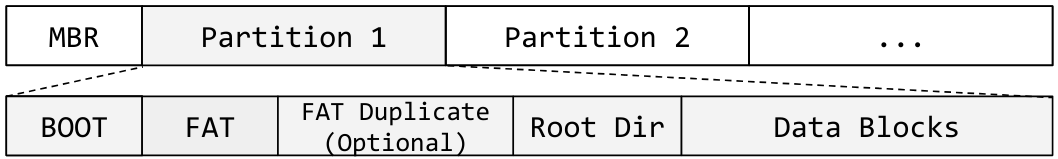
\includegraphics[scale=0.185]{fat-layout.png}
\begin{itemize}
	\item Size of FAT table: $2^{12}/2^{16}/2^{32}$ entries respectively
	\item FAT entry: either \texttt{FREE}, \texttt{EOF}, \texttt{BAD}, or block no.
	\item Larger cluster size $\rightarrow$ more internal fragmentation
\end{itemize}
\textbf{Largest Partition}: max cluster size = 32KB\\ 
\begin{tabular}{ |c|c|c| }
    \hline
	\textbf{FAT12} & \textbf{FAT16} & \textbf{FAT32} \\
	\hline
	$2^{12}$ clusters & $2^{16}$ clusters & $2^{28}$ clusters \\
	$2^{12}2^{15}$=128MB & $2^{16}2^{15}$=2GB & $2^{28}2^{15}$=8TB \\
	\hline
\end{tabular}
\textbf{Directory Structure}
\begin{itemize}
	\item Directories store in its data block a directory table of directory entries, each describing a file/subdir
	\item Free space must be calculated by gg through FAT
\end{itemize}
\textbf{Directory Entry (32 Bytes)}
\begin{itemize}
	\item Name (8) \& Extension (3): limited to 8+3 chars
	\item Attributes (1): indicate rdonly/hidden/archived
	\item Reserved (10): not actually used
	\item Creation Date (4): limited to 1980 to 2107
	\item First Block (2): 12/16/32 bits respectively
	\item File Size (4): theoretical $2^{32}=4$GB max file size; FAT16 limited to 2GB as max cluster size = 32KB
\end{itemize}
\textbf{File Deletion}
\begin{enumerate}
	\item Set first letter in name of directory entry to \texttt{0xE5}
	\item Set FAT to \texttt{FREE}; leave actual data blocks intact
\end{enumerate}

\medskip

{\small\textbf{Linux Ext2 File System}} \\
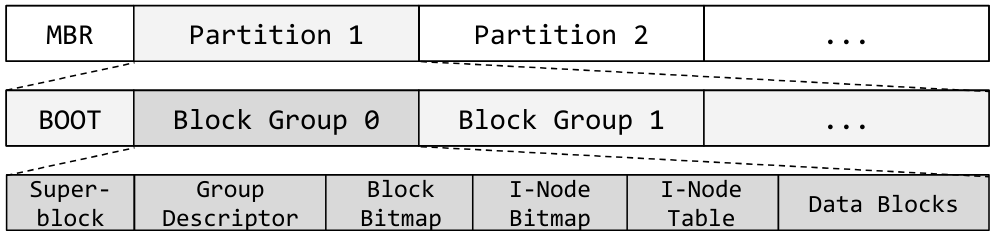
\includegraphics[scale=0.195]{ext2-layout.png}
\begin{itemize}
	\item \texttt{BOOT}: not used by linux, reserved for boot code
\end{itemize}
\textbf{Block Group Layout}
\begin{itemize}
	\item Superblock: layout of file system; number of inodes/disk blocks; start of free disk blocks
	\item Group Descriptor: location of bitmaps; number of free blocks/inodes; number of directories
	\item Bitmaps: 1-block long; tracks data block/inode usage; \texttt{1} = occupied, \texttt{0} = free; With 1KB data blocks, limited to 8192 number of data blocks/inodes
	\item Inode Table: array size limited by inode bitmap
	\item Data Blocks: non contiguous, stores all files/dir
\end{itemize}
\textbf{Inode (128 Bytes)}
\begin{itemize}
	\item Describes a file/dir's size, permission, ownership
	\item 12/1/1/1 data block pointers; an indirect block can contain $\frac{\text{size(data block)}}{\text{size(block ptr)}}$ number of pointers
	\item Inode is deleted only if ref count is 0
\end{itemize}
Given $m$B disk blocks and $32$ bit disk block address:
\begin{enumerate}
	\item A disk block address uses $\frac{32}{8} = 4$ bytes
	\item Indirect block can store $\frac{m}{4}$ addresses
	\item Max file size $= 12m + m\frac{m}{4} + m(\frac{m}{4})^2 + m(\frac{m}{4})^3$B
\end{enumerate}
\textbf{Directory Entry (Linked-List)}
\begin{itemize}
	\item Stored in data blocks of inodes describing a dir
\end{itemize}
An entry describes a file or a subdir, each with:
\begin{enumerate}
	\item Inode Number: \texttt{0} $\rightarrow$ unused; \texttt{2} $\rightarrow$ root dir
	\item Size of Entry: to locate next entry
	\item Length: of name of file/subdirectory
	\item Type: file or subdirectory or others
	\item Name: up to 255 characters; OS linearly searches this field to get corresponding inode number (slow)
\end{enumerate}
\begin{tabular}{ |c|c| }
    \hline
	\textbf{Symbolic Link} & \textbf{Hard Link} \\
	\hline
	A new inode/file & A directory entry \\
	Contain pathname of TF & *Point to TF's inode \\
	Search for TF's inode & Just use inode ref \\
	Can link to dir & Cannot link to dir \\
	Can link across FS & Cannot link across FS \\
	\hline
\end{tabular}
\textbf{*}If TF is deleted, HL will still work, but SL will not



\begin{center}
    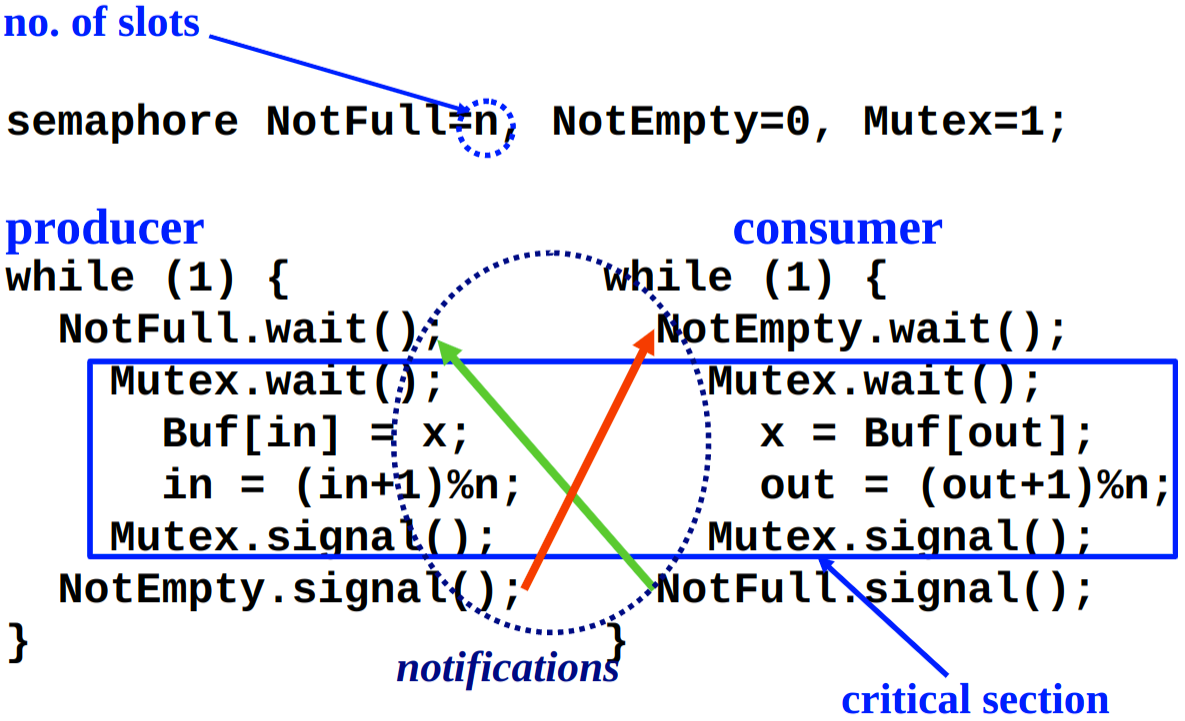
\includegraphics[scale=0.13]{producer-consumer.png}    
\end{center}
% \begin{center}
%     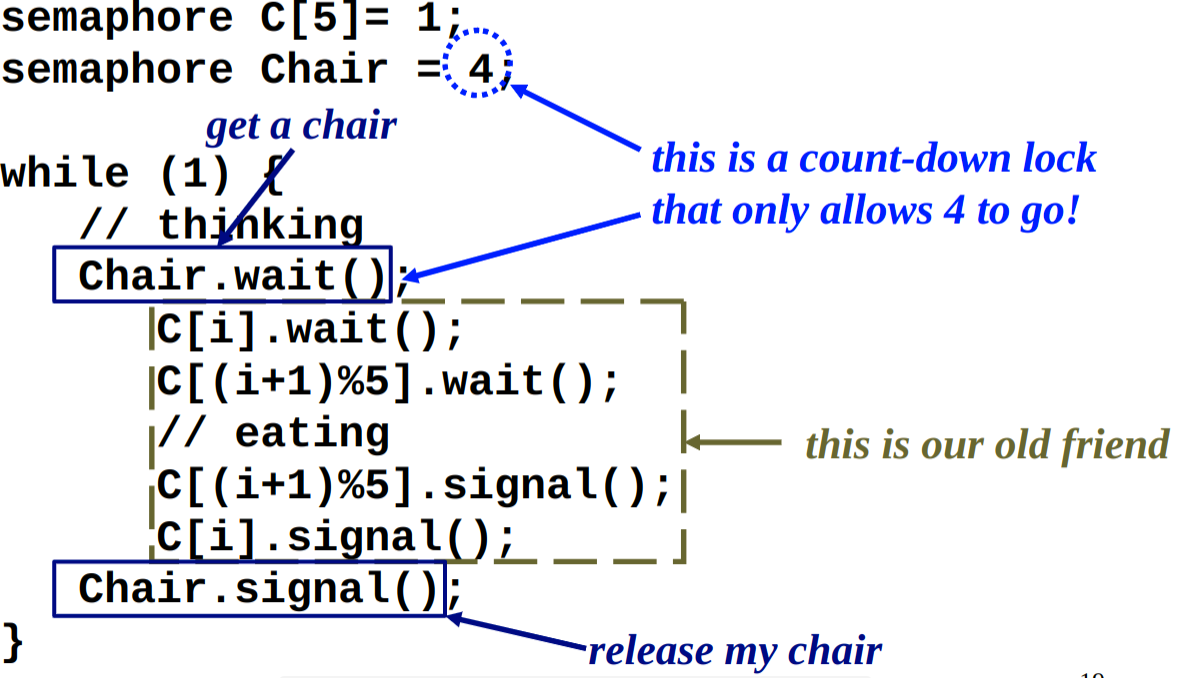
\includegraphics[scale=0.14]{philosophers-countdown.png}
% \end{center}
\begin{center}
    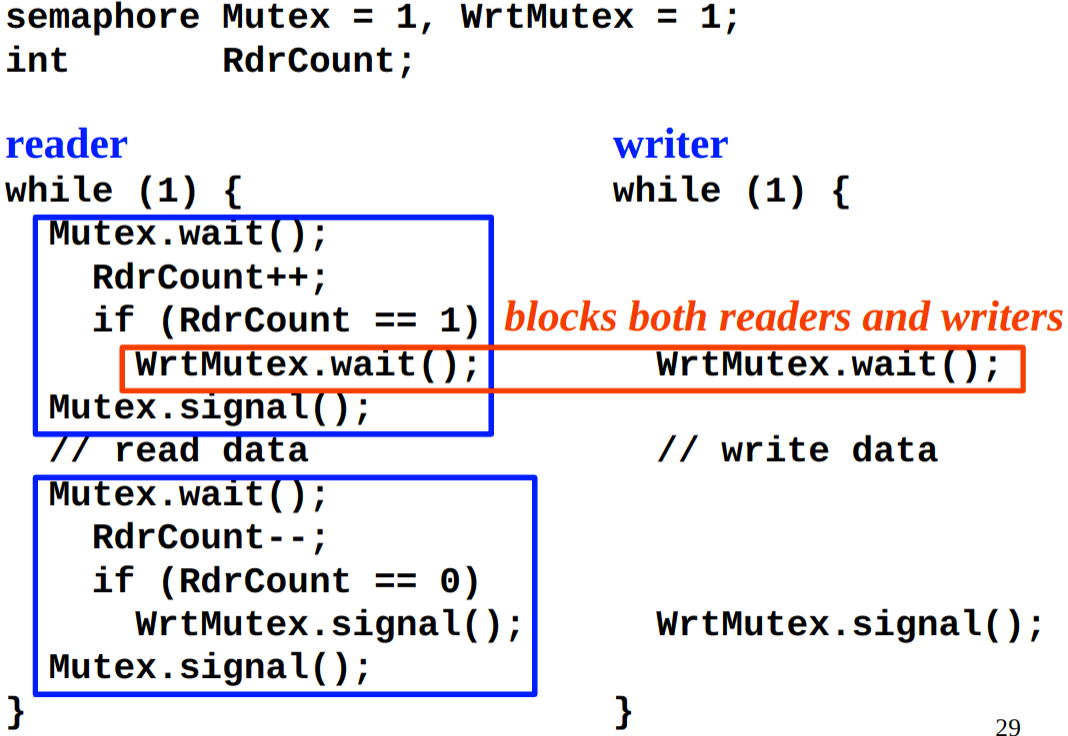
\includegraphics[scale=0.14]{readers-writers.png}
\end{center}


\end{multicols*}
\end{document}
